\documentclass{revtex4}
\usepackage{hyperref}
\usepackage{graphicx}
\begin{document}

\title[scater supplementary figures]{Supplementary Figures---``\emph{scater:} pre-processing, quality control, normalisation and visualisation of single-cell RNA-seq data in R''}
\author{Davis J.~McCarthy\,$^{\text{1,2,4,6}*}$, Kieran R.~Campbell\,$^{\text{2,5}}$, Aaron T.~L.~Lun\,$^{\text{7}}$ and Quin F.~Wills\,$^{\text{2,3}}$}
\address{$^{\text{1}}$European Molecular Biology Laboratory - European Bioinformatics Institute (EMBL-EBI), Hinxton CB10 1SD, Cambridgeshire, UK;\\
$^{\text{2}}$Wellcome Trust Centre for Human Genetics, University of Oxford,
Oxford, Oxfordshire, UK;\\
$^{\text{3}}$ Weatherall Institute for Molecular Medicine, University of Oxford, Oxford, Oxfordshire, UK;\\
$^{\text{4}}$Department of Statistics, University of Oxford, Oxford, Oxfordshire, UK;\\
$^{\text{5}}$Department of Anatomy, Physiology and Genetics, University of Oxford, Oxford, Oxfordshire, UK;\\
$^{\text{6}}$St Vincent's Institute of Medical Research, 41 Victoria Parade Fitzroy Victoria 3065, Australia; and \\
$^{\text{7}}$CRUK Cambridge Institute, Robinson Way, Cambridge CB2 0RE,
Cambridgeshire, UK.}

\begin{abstract}
Supplementary Figures---an overview of the SCESet class; an overview of the \emph{scater} ecosystem; examples of using the \emph{scater} GUI.\\ \\
\textbf{Contact:} \href{davis@ebi.ac.uk}{davis@ebi.ac.uk}
\end{abstract}


\maketitle


\section*{Supplementary Figures}


\begin{figure}[!tpb]%figure2
\centerline{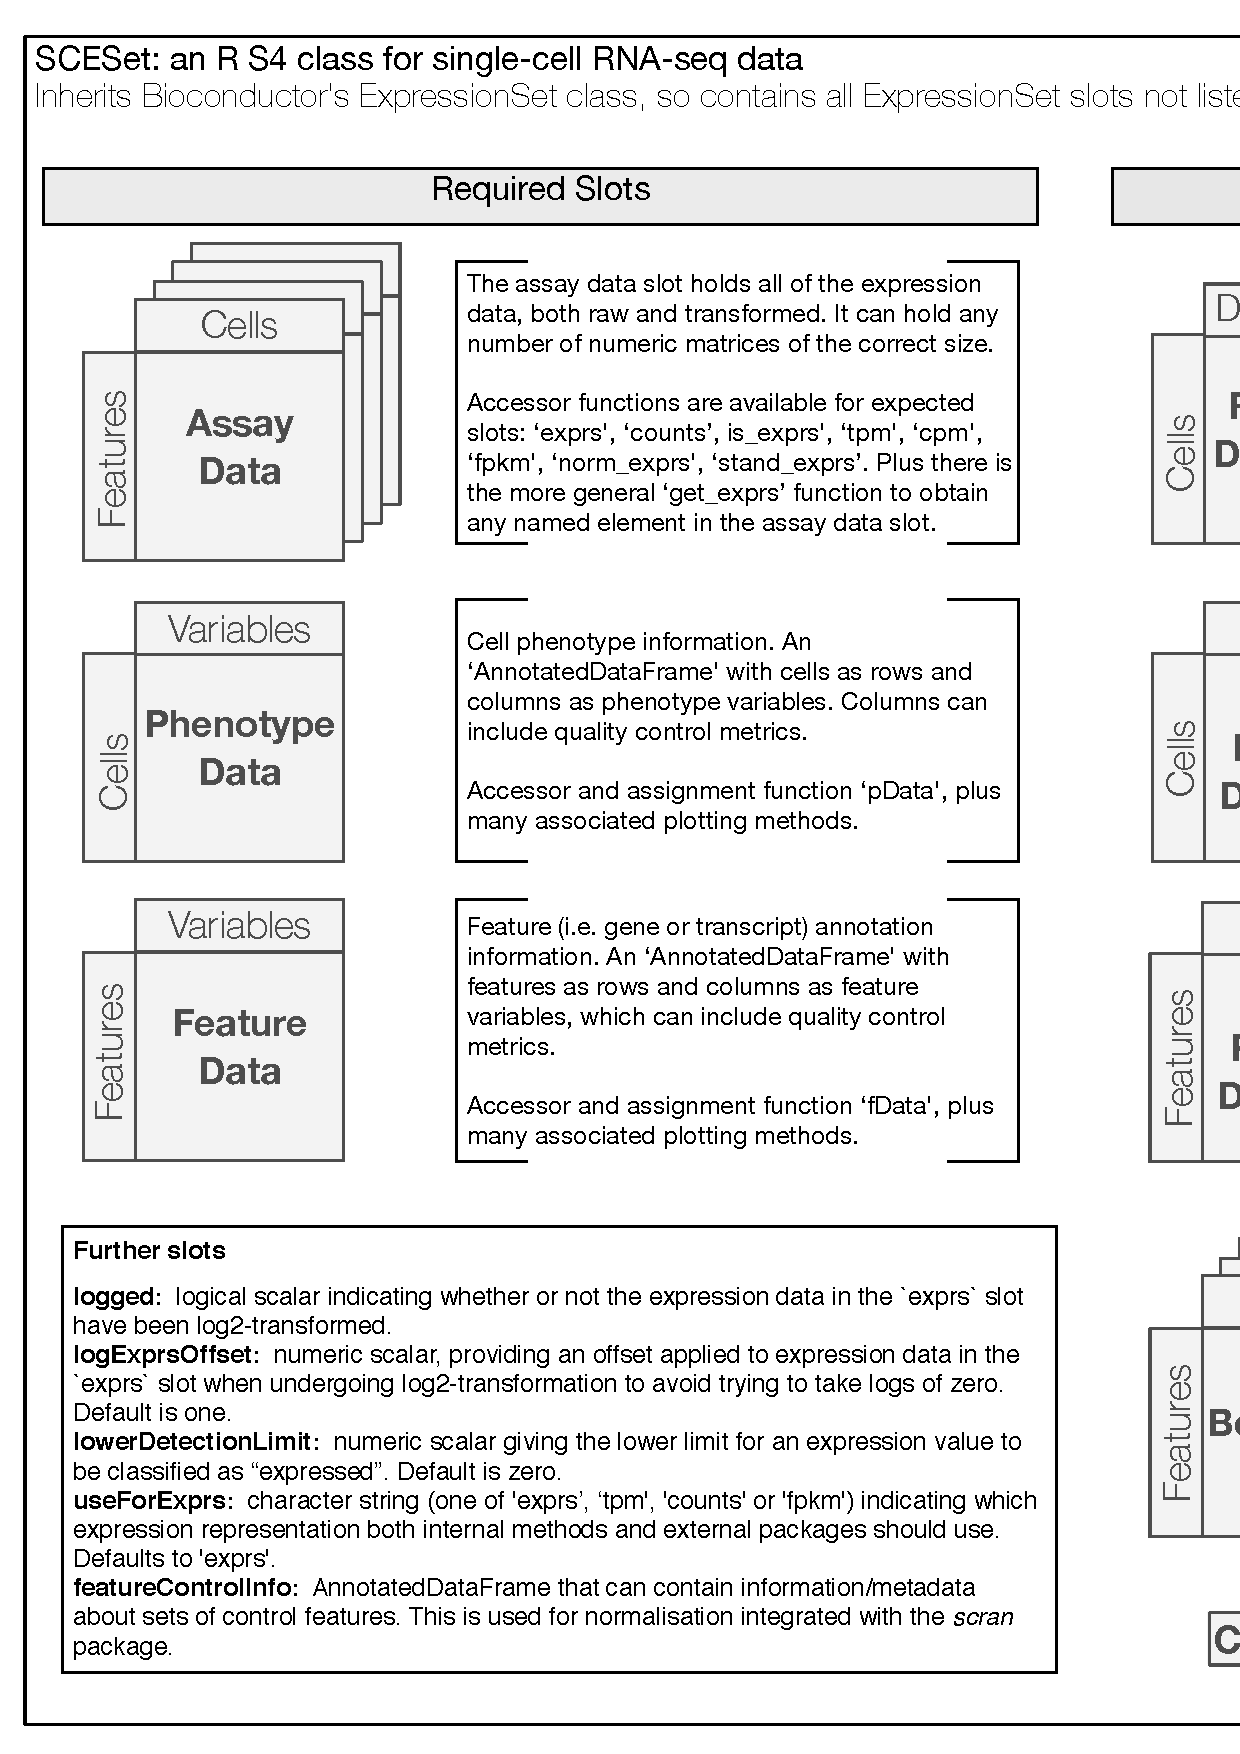
\includegraphics[width=0.95\textwidth]{figures/sceset_outline.pdf}}
\caption{An overview of the SCESet class that underpins the \emph{scater} package. Building on Bioconductor's ExpressionSet class, it is a fully-featured, sophisticated and flexible data class tailored to scRNA-seq data.}\label{fig:02}
\end{figure}


\begin{figure}[!tpb]
\centerline{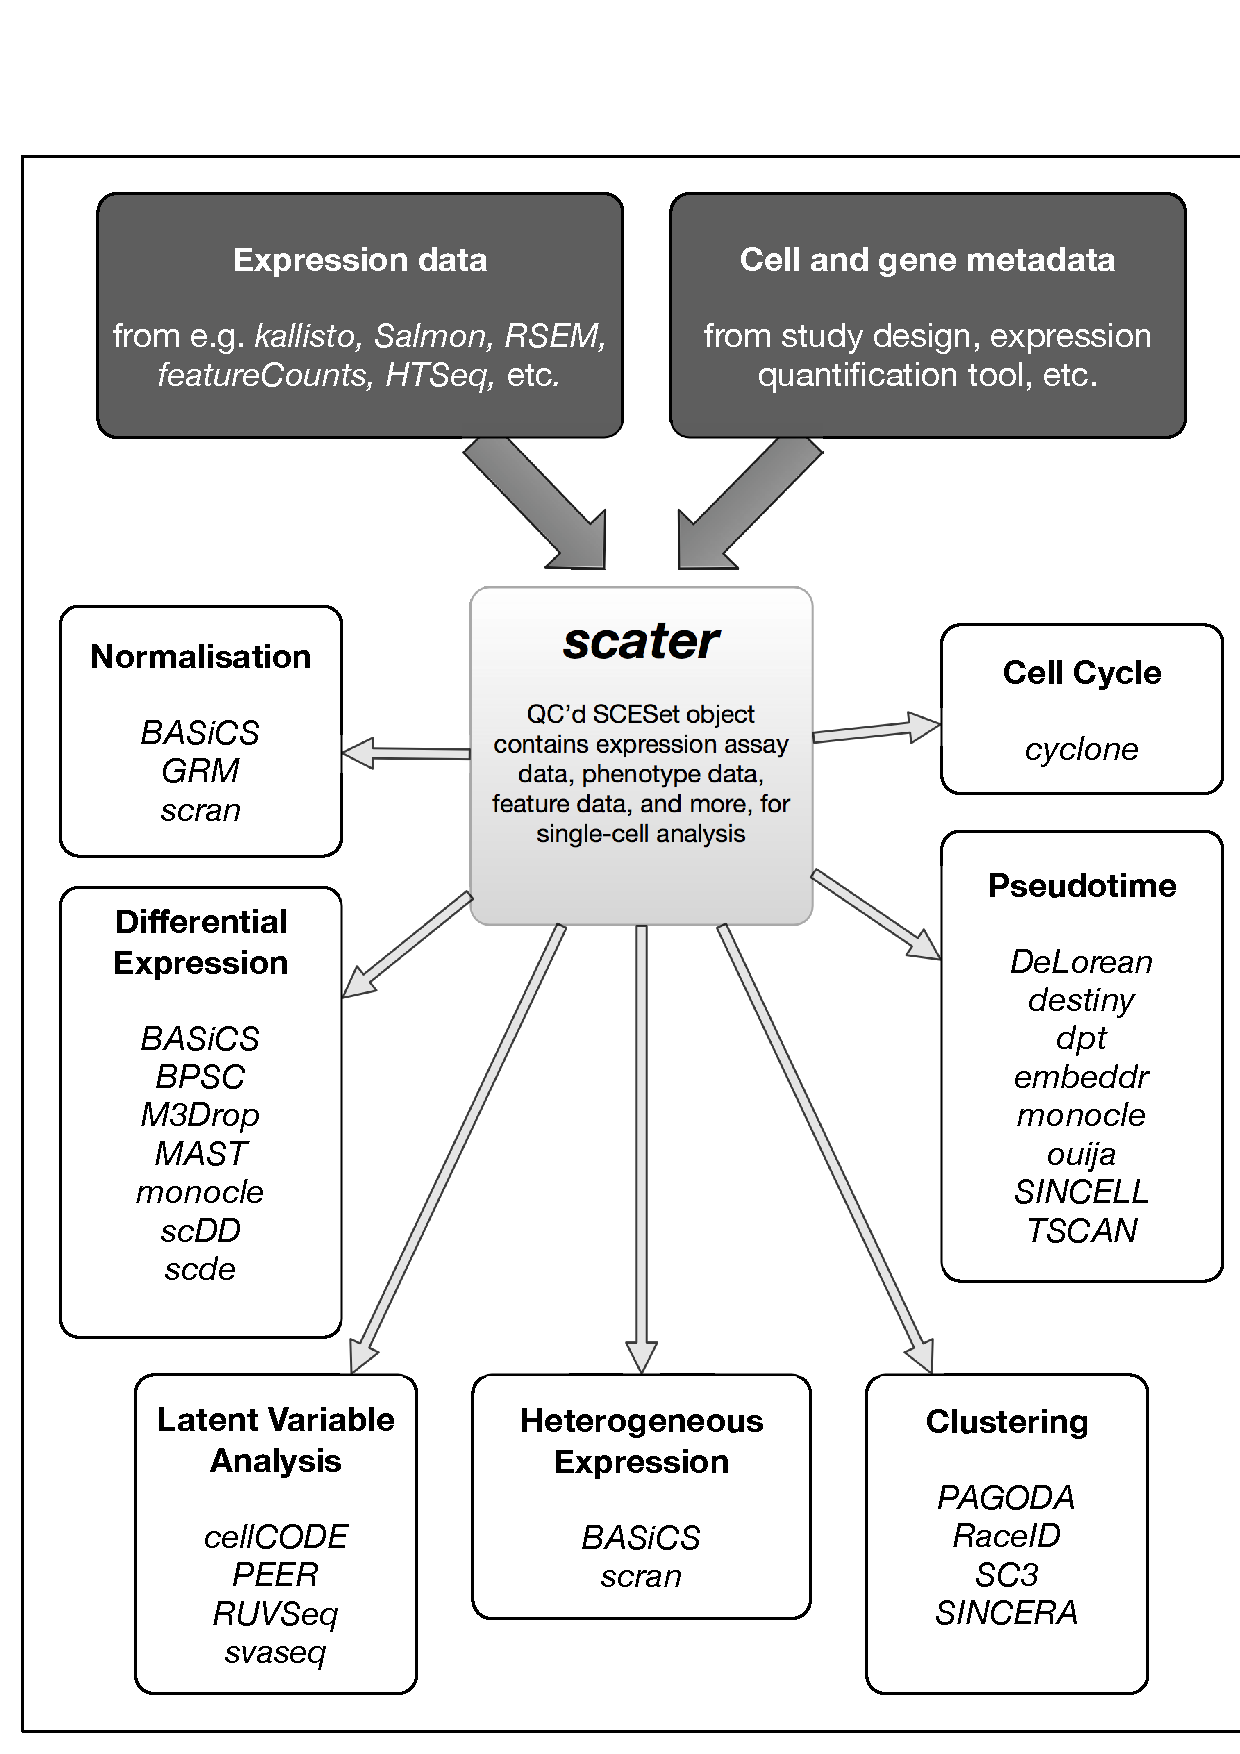
\includegraphics[width=0.95\textwidth]{figures/scater_ecosystem.pdf}}
\caption{An overview of the \emph{scater} ecosystem. The SCESet class in \emph{scater} acts as a convenient hub for datasets so that many other methods and tools implemented in R can be applied.}\label{fig:scater-eco}
\end{figure}


\begin{figure}[!tpb]
\centerline{\includegraphics[width=0.95\textwidth]{figures/scater_gui_landing_page.pdf}}
\caption{The landing page for the \emph{scater} graphical user interface (GUI).}\label{fig:scater-gui-landing}
\end{figure}


\begin{figure}[!tpb]
\centerline{\includegraphics[width=0.95\textwidth]{figures/scater_gui_plotqc.pdf}}
\caption{The \texttt{plotQC} page for the \emph{scater} graphical user interface (GUI).}\label{fig:scater-plotqc}
\end{figure}


\begin{figure}[!tpb]
\centerline{\includegraphics[width=0.95\textwidth]{figures/scater_gui_pca_qc.pdf}}
\caption{The \texttt{plotPCA - QC} page for the \emph{scater} graphical user interface (GUI).}\label{fig:scater-pca-qc}
\end{figure}


\section*{Details of package dependencies}

The package builds on many other R packages: \emph{Biobase} and \emph{BiocGenerics} for core Bioconductor functionality  \citep{Huber2015-en}; \emph{plyr} \citep{Wickham2015-kj}, \emph{reshape2} \citep{Wickham2012-ec}, \emph{dplyr} \citep{Wickham2015-la}, \emph{data.table} \citep{Dowle2015-zc} and \emph{magrittr} \citep{Bache2014-sa} for reading and
tidying data; \emph{ggplot2} \citep{Wickham2016-dc} for plotting; \emph{biomaRt} \citep{Durinck2005-yz} for feature annotation; \emph{edgeR} \citep{Robinson2010-ky} for computation of normalisation size factors and counts-per-million values; \emph{limma} \citep{Ritchie2015-so} for efficient fitting of linear models to features; \emph{rhdf5} \citep{Fischer2016-me}, \emph{rjson} \citep{Couture-Beil2014-kk} and \emph{tximport} \citep{Soneson2015-fw} for reading in transcript-level expression values;
\emph{viridis} \citep{Garnier2016-hk} for perceptually-uniform colour
maps for plotting; \emph{parallel} for parallel computation; \emph{matrixStats} \citep{Bengtsson2016-tn} for computation of summary statistics from matrices; \emph{cowplot} \citep{Wilke2016-hj} for attractive plotting themes; \emph{destiny} \citep{Angerer2015-sw} for producing diffusion maps; \emph{Rtsne} \citep{Krijthe2015-is} for producing t-SNE plots; \emph{mvoutlier}
\citep{Filzmoser2015-kx} for multivariate outlier detection from PCA of QC metrics; \emph{roxygen2} \citep{Wickham2015-pu}, \emph{BiocStyle} \citep{Huber2015-en}, \emph{knitr} \citep{Xie2013-bn} and \emph{rmarkdown} \citep{Allaire2016-dl} for generating documentation; and \emph{testthat} \citep{Wickham2011-cj} for unit testing. As well as functioning in the usual R environments, \emph{scater} also has a GUI built using
\emph{shiny} \citep{Chang2016-of} and \emph{shinydashboard} \citep{Chang2015-bn} for intuitive and interactive data visualisation. Calling the \verb|scater_gui| function from within an R session opens up the GUI in a web browser.


\bibliographystyle{natbib}
%\bibliographystyle{achemnat}
%\bibliographystyle{plainnat}
%\bibliographystyle{abbrv}
%\bibliographystyle{plain}
%\bibliographystyle{bioinformatics}
\bibliography{main}


\end{document}
